%% bare_conf.tex
%% V1.3
%% 2007/01/11
%% by Michael Shell
%% See:
%% http://www.michaelshell.org/
%% for current contact information.
%%
%% This is a skeleton file demonstrating the use of IEEEtran.cls
%% (requires IEEEtran.cls version 1.7 or later) with an IEEE conference paper.
%%
%% Support sites:
%% http://www.michaelshell.org/tex/ieeetran/
%% http://www.ctan.org/tex-archive/macros/latex/contrib/IEEEtran/
%% and
%% http://www.ieee.org/

%%*************************************************************************
%% Legal Notice:
%% This code is offered as-is without any warranty either expressed or
%% implied; without even the implied warranty of MERCHANTABILITY or
%% FITNESS FOR A PARTICULAR PURPOSE! 
%% User assumes all risk.
%% In no event shall IEEE or any contributor to this code be liable for
%% any damages or losses, including, but not limited to, incidental,
%% consequential, or any other damages, resulting from the use or misuse
%% of any information contained here.
%%
%% All comments are the opinions of their respective authors and are not
%% necessarily endorsed by the IEEE.
%%
%% This work is distributed under the LaTeX Project Public License (LPPL)
%% ( http://www.latex-project.org/ ) version 1.3, and may be freely used,
%% distributed and modified. A copy of the LPPL, version 1.3, is included
%% in the base LaTeX documentation of all distributions of LaTeX released
%% 2003/12/01 or later.
%% Retain all contribution notices and credits.
%% ** Modified files should be clearly indicated as such, including  **
%% ** renaming them and changing author support contact information. **
%%
%% File list of work: IEEEtran.cls, IEEEtran_HOWTO.pdf, bare_adv.tex,
%%                    bare_conf.tex, bare_jrnl.tex, bare_jrnl_compsoc.tex
%%*************************************************************************

% *** Authors should verify (and, if needed, correct) their LaTeX system  ***
% *** with the testflow diagnostic prior to trusting their LaTeX platform ***
% *** with production work. IEEE's font choices can trigger bugs that do  ***
% *** not appear when using other class files.                            ***
% The testflow support page is at:
% http://www.michaelshell.org/tex/testflow/



\documentclass[conference]{IEEEtran}
% Add the compsoc option for Computer Society conferences.
%
% If IEEEtran.cls has not been installed into the LaTeX system files,
% manually specify the path to it like:
% \documentclass[conference]{../sty/IEEEtran}


% Some very useful LaTeX packages include:
% (uncomment the ones you want to load)

% *** GRAPHICS RELATED PACKAGES ***
%
\usepackage[pdftex]{graphicx}

% *** MATH PACKAGES ***
%
\usepackage[cmex10]{amsmath}

% *** SUBFIGURE PACKAGES ***
%\usepackage[tight,footnotesize]{subfigure}
% subfigure.sty was written by Steven Douglas Cochran. This package makes it
% easy to put subfigures in your figures. e.g., "Figure 1a and 1b". For IEEE
% work, it is a good idea to load it with the tight package option to reduce
% the amount of white space around the subfigures. subfigure.sty is already
% installed on most LaTeX systems. The latest version and documentation can
% be obtained at:
% http://www.ctan.org/tex-archive/obsolete/macros/latex/contrib/subfigure/
% subfigure.sty has been superceeded by subfig.sty.



%\usepackage[caption=false]{caption}
\usepackage[font=footnotesize,caption=false]{subfig}
% subfig.sty, also written by Steven Douglas Cochran, is the modern
% replacement for subfigure.sty. However, subfig.sty requires and
% automatically loads Axel Sommerfeldt's caption.sty which will override
% IEEEtran.cls handling of captions and this will result in nonIEEE style
% figure/table captions. To prevent this problem, be sure and preload
% caption.sty with its "caption=false" package option. This is will preserve
% IEEEtran.cls handing of captions. Version 1.3 (2005/06/28) and later 
% (recommended due to many improvements over 1.2) of subfig.sty supports
% the caption=false option directly:
%\usepackage[caption=false,font=footnotesize]{subfig}
%
% The latest version and documentation can be obtained at:
% http://www.ctan.org/tex-archive/macros/latex/contrib/subfig/
% The latest version and documentation of caption.sty can be obtained at:
% http://www.ctan.org/tex-archive/macros/latex/contrib/caption/


% --------------- USEPACKAGE agregados por guanucoluis ----------------

\usepackage[utf8]{inputenc}
\usepackage{multirow}
%\usepackage[english]{babel}
\usepackage{amssymb}
%\usepackage[pdftex]{graphicx}
\usepackage[hyphenbreaks]{breakurl}
\usepackage[hyphens]{url}
\usepackage{lipsum}
\usepackage{listings}
\lstset{% general command to set parameter(s)
basicstyle=\scriptsize\ttfamily}

\usepackage{textcomp}

% ------------------------- Agregados por maxi ------------------------

\renewcommand{\abstractname}{Resumen}
\renewcommand{\IEEEkeywordsname}{Palabras claves}
\renewcommand{\figurename}{Fig.}
\renewcommand{\tablename}{Tabla}
\renewcommand{\refname}{Referencias}
\hyphenation{de-sa-rro-llar de-sa-rro-llos}

%lista de posibles "Fixed names"  de latex que pueden hacer falta
%\abstractname	 Abstract
%\alsoname	 see also (makeidx package)
%\appendixname	 Appendix
%\bibname	 Bibliography (report,book)
%\ccname	 cc (letter)
%\chaptername	 Chapter (report,book)
%\contentsname	 Contents
%\enclname	 encl (letter)
%\figurename	 Figure (for captions)
%\headtoname	 To (letter)
%\indexname	 Index
%\listfigurename	 List of Figures
%\listtablename	 List of Tables
%\pagename	 Page (letter)
%\partname	 Partnnn
%\refname	 References (article)
%\seename	 see (makeidx package)
%\tablename	 Table (for caption)



% correct bad hyphenation here
\hyphenation{op-tical net-works semi-conduc-tor}

\begin{document}
%
% paper title
% can use linebreaks \\ within to get better formatting as desired
\title{Filtro digital reconfigurable basado en FPGA}

% author names and affiliations
% use a multiple column layout for up to three different
% affiliations
\author{\IEEEauthorblockN{Franco Bocalon, Luis Guanuco, Santiago
    Nolasco}
  \IEEEauthorblockA{Procesamiento Digital de Señales\\
    Especialidad en Sistemas Embebidos\\
    Instituto Universitario Aeronáutico}
}

% use for special paper notices
%\IEEEspecialpapernotice{(Invited Paper)}


% make the title area
\maketitle


\begin{abstract}
  La flexibilidad que proporciona el dominio digital en lo que
  respecta a la síntesis de filtros se ha incrementado para mejor con las
  nuevas tecnologías. La alta velocidad de procesamiento de los 
  microcontroladores de bajo costo y el acceso a plataformas basadas
  en FPGA permiten completar el estudio en profundidad de los filtros
  digitales. Aquí se presenta una implementación de un filtro FIR
  reconfigurable con la integración de diferentes software utilizados
  en el módulo \emph{Procesamiento de Señales Digitales}.
\end{abstract}

% Note that keywords are not normally used for peerreview papers.
\begin{IEEEkeywords}
DSP, FIR filter, FPGA, soft-core 
\end{IEEEkeywords}

% IEEEtran.cls defaults to using nonbold math in the Abstract.
% This preserves the distinction between vectors and scalars. However,
% if the conference you are submitting to favors bold math in the abstract,
% then you can use LaTeX's standard command \boldmath at the very start
% of the abstract to achieve this. Many IEEE journals/conferences frown on
% math in the abstract anyway.

% no keywords

% For peer review papers, you can put extra information on the cover
% page as needed:
% \ifCLASSOPTIONpeerreview
% \begin{center} \bfseries EDICS Category: 3-BBND \end{center}
% \fi
%
% For peerreview papers, this IEEEtran command inserts a page break and
% creates the second title. It will be ignored for other modes.
\IEEEpeerreviewmaketitle

\section{Introducción}

Con el objeto de analizar el comportamiento de los filtros
digitales,se implementan  cuatro tipos de filtros: \emph{pasa-bajo},
\emph{pasa-alto}, \emph{pasa-banda} y \emph{suprime-banda} según los
siguientes requerimientos:

\begin{itemize}
\item  Orden del filtro N=12
\item Longitud de palabra 13 bits
\item Pequeña interfaz de usuario para elegir y cargar los coeficientes
  en la plataforma embebida a traves del puerto serie.
\end{itemize}

\section{Modulado}
\label{sec:mod}

Para poder tener los coeficientes necesarios para la implementacion de
un filtro FIR se utilizo la herramienta \emph{FDATool} del paquete
\emph{MathWorks}. La principal característica de estos filtros es un
número finito de términos no nulos como respuesta a una señal impulso.

FDATool permite seleccionar el tipo de filtro, orden y ventana a
implementar. En nuestro caso el tipo de ventana seleccionada es la
Kaiser. Ésta proporciona un mejor control de la pendiente y
perturbación en la banda de paso. 

\begin{figure}[!t]
\centering
  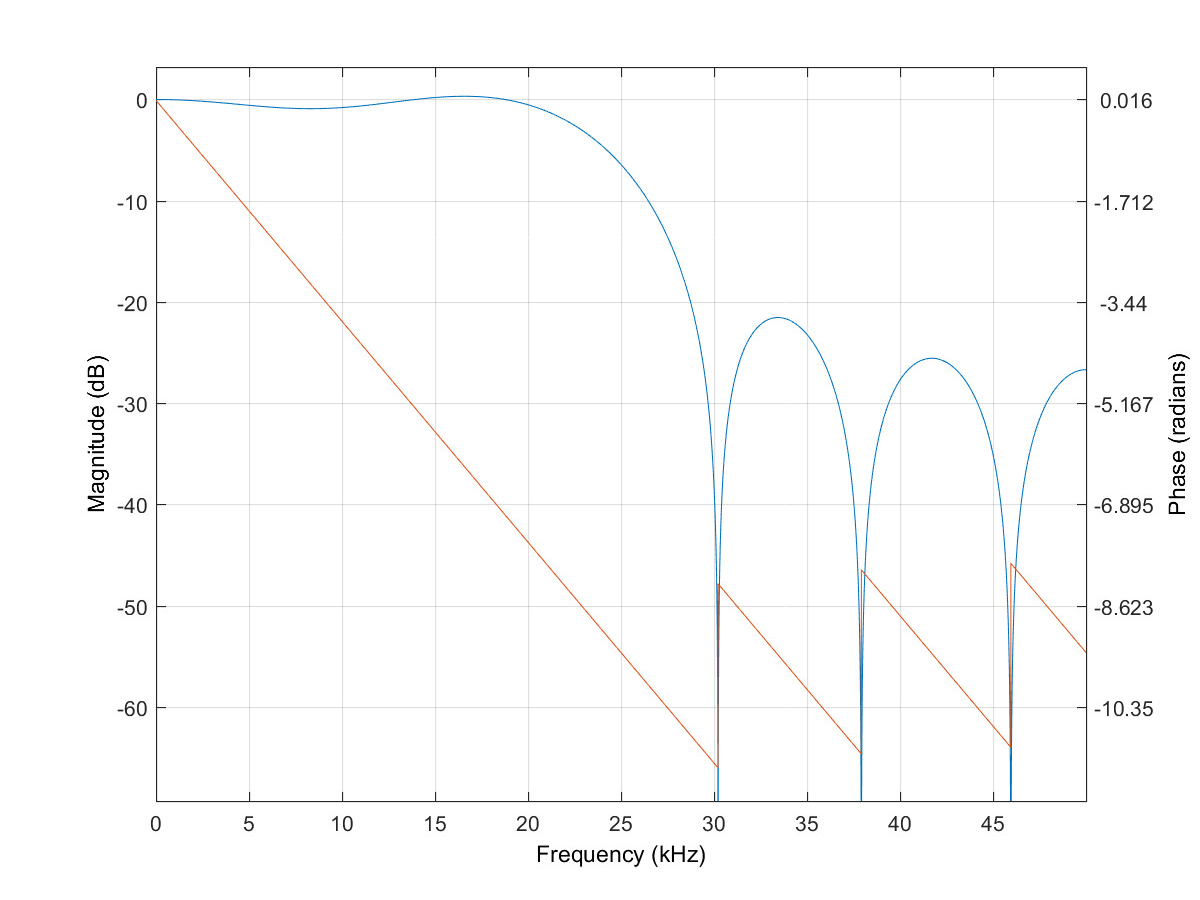
\includegraphics[width=0.5\textwidth]{images/fdatool-plot}
  \caption{Respuesta en frecuencia y fase del filtro sintetizado por TDATool.}
  \label{fig:res-fil}
\end{figure}

En la Figura \ref{fig:res-fil}  se puede apreciar la respuesta del
filtro. Claramente se observa la frecuencia de corte y los lóbulos
atenuados para las frecuencias mayores en el caso del filtro pasa
bajo.La amplitud de ganancia esta indicada con color azul y la fase en
rojo, es muy importante de destacar que en estos filtros se pueden
diseñar si asi el diseño lo requiera,  una respuesta de fase lineal.


Una vez generados los coeficientes, disponibles en un
array en el workspace de MATLAB, pueden ser  enviados a la plataforma
embebida (basada en una FPGA). Se deben cuantizar los coeficientes, es decir
enviarlos en el formato de palabra de trabajo de la placa, en nuestro
caso particular 16bits sin signo. Por lo tanto los generados
coeficientes por FDATool tienen que ser convertidos desde punto flotante
a punto fijo y cambiar el tipo de notación con signo a sin signo. 
Esta conversión se realizo a través del siguiente algoritmo escrito en
un script de MATLAB.
\begin{lstlisting}[frame=single]
%%%%%%FiltroV1%%%%
  clc
  close all
  delete(instrfind({'Port'},{'/dev/ttyUSB1'}));
  
  condition = 1;
  while condition
  % do something
  nroFiltro = input ('Elija su filtro: 1_Pbajo 
  2_Palto 3_Pbanda 4_Sbanda\n');
  if((nroFiltro < 5)&&(nroFiltro > 0))
  condition=0;
  end 
  end
  % Signal inputs
  % u = evalin( 'base', 'Num' )
  switch nroFiltro
  case 1
  u=Num;
  case 2
  u=Num1;
  case 3
  u=Num2;
  case 4   
  u=Num3;
  otherwise;
  end
\end{lstlisting}
El cual consta de una minima interfaz grafica que permite al usuario
elegir que filtro quiere implementar en la FPGA y luego enviarlo a
traves de un puerto estandar RS232.

\begin{lstlisting}[frame=single]
  FM=10;
  Mayor=max(u)*FM;
  Normal=u*1000;
  Bits=12;
  Normal=round(Normal);
  Q=quantizer('fixed','round','saturate',[Bits 0]);
  hexh=num2hex(Q,Normal);
  Binario=num2bin(Q,Normal);
  Entero= num2int(Q,Normal);
  h=hex2dec(hexh);
  l=bin2dec(Binario);
  % Vector cuantizado 1x13
  % VectorCoef = quantize (Vector,1,13,0); % Con siNumgno, 
  % 13bits y sin fraccional
\end{lstlisting}

\begin{lstlisting}[frame=single]
  % Trasmision serie
  s=serial('/dev/ttyUSB1');%se crea un objeto del puerto
  s.Baudrate=115200;      % configuracion puerto
  s.DataBits=8;
  s.Parity='none';
  s.StopBits=1;
  s.FlowControl='none';
  s.RequestToSend='off';
  s.OutputBufferSize=14;  % es el numero de bytes a enviar
  s.InputBufferSize=14; % es el numero de bytes a recibir
  s.Timeout=5;            % 5 segundos de tiempon de espera
  set(s,'Terminator','CR/LF');% caracter fin de envio  
  fopen(s);               % se abre el objeto  
  % FIR COEFF
  % Escritura de bytes iniciales para
  % iniciar la conversion en la fpga
  K1= [];  
  fwrite(s,250,'uint8'); %tx 0xFA bit menos significativos  
  fwrite(s,255,'uint8'); %tx 0xFF  
  K1 = [K1 fread(s,1,'uint16')];  
  i=0;
  for i=1:length(l);
  fwrite(s,l(i),'uint16');   % se envia entero sin signo de 8 bits
  K1 = [K1 fread(s,1,'uint16')];
  end  
  fclose(s); 
  delete (s);
  clear s;
\end{lstlisting}


Se utilizaron  funciones propias de MATLAB
para cuantizar y convertir los coeficientes negativos a sin
signo. Por último, es interesante destacar que eligiendo el número de
coefcientes par o impar podemos tener una simetría o asimetría en los
valores de los coeficientes, por ejemplo el filtro pasa-bajo es con
todos los coeficientes positivos y con pariedad.

\section{Implementación}
\label{sec:imp}

Se utiliza la plataforma \emph{BASYS2} y los módulos \emph{PmodAD1} y
\emph{PmodDA2}, todos fabricados por Digilent
Inc.\footnote{\burl{https://digilentinc.com/}}. 

\section{Conclusiones}
\label{sec:con}
\lipsum[87]

\begin{thebibliography}{1}

\bibitem{SOA2}
  Umair~Ashraf, \emph{CS 415 N-Tier Application Development}. National
  University of Computer and Emerging Sciences. July 5, 2013.

\bibitem{NordicAPIs}
Bruno~Pedro, \emph{Is REST better than SOAP? Yes, in Some Use Cases},
url:
\texttt{\burl{http://nordicapis.com/rest-better-than-soap-yes-use-cases/}}.

\end{thebibliography}

% that's all folks
\end{document}


